%%%%%%%%%%%%%%%%%%%%%%%%%%%%%%%%%%%%%%%%%%%%%%%%%%%%%%%%%%%%%%%%%%%
% Background
% Team:
% Wolverine
% Members: 
% Dexter Chen, Eric Chang, Eric Lee, Jacky Wu, Karthick Mani, Kenvin Lo, Yu-cheng Chen
% Relative files:
% Main.tex, Background_Wolverine.tex, Library.bib, Wolverine_Background_Chart_1.png
% Note: 
% Do not compile this file compile Main.tex to get the pdf file instead.
%%%%%%%%%%%%%%%%%%%%%%%%%%%%%%%%%%%%%%%%%%%%%%%%%%%%%%%%%%%%%%%%%%%
	
\subsection{Information retrieval on existing database}
\textit{\footnotesize Author:Dexter Chen, Eric Chang, Eric Lee, Jacky Wu, Karthick Mani, Kenvin Lo, Yu-cheng Chen.}\\

We live in the time where technologies evolve beyond our imagination.
Information growth in a exponential rate according to \cite{Tague1981}, thus we can't rely on the old fashion ways to find data. 
We need new information retrieval methods to handle such a big amount of data.
But most of the information retrieval methods such as search engine can't really search everything on the web. 
They can only search the data that has been captured into the database according to \cite{Grehan2002}. 
Thus, we need to create a database to store these data and automatically update them frequently.

There are several online libraries currently available for us to get the academic articles we need.
And they can be roughly divided into three group according to the way they store articles base on the division used by National Taiwan University Library.

\paragraph{Index libraries}

	These kind of libraries stores the index and abstract of the articles.
	They don't provide the full-text documents directly, but may give the linkage to the publisher websites of articles.
	And can be categorized by the type of articles they include.
	
	\begin{itemize}
		
		\item\textbf{Comprehensive topics}\\Libraries such as Web of Science, Scopus...
		\item\textbf{Specialized topics}\\Libraries such as Compendex, BIOSIS Previews, PubMed...
		
	\end{itemize}
	
\paragraph{Publisher libraries}

	These libraries are created by the publishers themselves, so they provide the newest and complete documents directly.
	And can also be categorize by the type of articles they include.
	
	\begin{itemize}
		
		\item\textbf{Comprehensive topics}\\Libraries such as Science Direct, Springer Link, Wiley Online Library...
		\item\textbf{Specialized topics}\\Libraries such as Nature.com, Emerald Management Xtra, IEEE Xplore...
		
	\end{itemize}
	
\paragraph{Aggregator libraries}

	These libraries do not publish the articles by themselves, but they still sometimes provide the full-text articles to the user.
	The way they do this is to negotiate with some of the publisher libraries and get the authorization of the articles.
	Libraries such as EBSCOhost, ProQuest, JSTOR...

The comparison between three kinds of library can be found on Figure \ref{WBC1}. 
On the next section we'll discuss about more details about some of the existing libraries.

\subsubsection{Introduction to several libraries }\todo{Consider to change the title.}

\begin{enumerate}
	
	\item\textbf{PubMed}
	\setlength{\parindent}{1em}
		
	 PubMed is a free library which is used for searching reference papers and abstracts related to the biomedical topics.
	 PubMed’s design philosophy is based on full-text XML files, which are readable by both the machines, humans and moreover technology independent.
	 PubMed is classified into Index libraries, which is the prime reason that it won’t be able to provide full text in some papers.
	 For the type of database used by PubMed is Microsoft SQL server, which is a relational database to store all of the archives such as XML, images, PDF files supplementary, etc. \todo{Good that you start by describing what it is and then tell how it is built.}
		
	\item\textbf{IEEE Xplore}
	\setlength{\parindent}{1em}
	
	IEEE Xplore is a scholarly research library formerly known as IEEE/IET Electronic Library (IEL).
	The IEEE is an acronym for Institute of Electrical and Electronics Engineers, which is one of the leading standard organizations in the world.
	More than 3.5-million full-text documents in the field of electrical, engineering, computer science and electronics are provided in this library. 
	
	The front and user interface of IEEE library present the information on the screen, including the latest Angular, Jquery, HTML 5, CSS, etc.\todo{You mean it is implemented using these techniques. Please don't use etc. when you describe how something is built and do it in this context.} 
	Most of the HTML for PDF, either it is for journal (conference) articles or standards get dynamic transformations real time and served through MarkLogic.
	Endeca, which is an Oracle product powers Xplore searches, is used in the search layer.
	All PDF files are fed through Endeca system.
	Endeca servers will provide the matching documents and Xplore platform presents it on the screen to the user.
	And all the content is stored in oracle metadata which will be consumed by Endeca, MarkLogic Authentication, and Authorization services.
	
	\item\textbf{EBSCOhost}
	\setlength{\parindent}{1em}
	
		
		EBSCO Information Services, 
		headquartered in Ipswich, 
		Massachusetts, 
		is a division of EBSCO Industries Inc., 
		the third largest private company in Birmingham, 
		Alabama, 
		with annual sales of nearly $2 billion according to the BBJ's 2013 Book of Lists.
		[1] EBSCO offers library resources to customers in academic, 
		medical, 
		K–12, 
		public library, 
		law, 
		corporate, 
		and government markets. 
		Its products include EBSCONET, 
		a complete e-resource management system, 
		and EBSCOhost, 
		which supplies a fee-based online research service with 375 full-text databases, 
		a collection of 600,000-plus ebooks, 
		subject indexes, 
		point-of-care medical references, 
		and an array of historical digital archives. 
		In 2010, 
		EBSCO introduced its EBSCO Discovery Service (EDS) to institutions, 
		which allows searches of a portfolio of journals and magazines.[2]
		
		EBSCO Information Services is a division of EBSCO Industries Inc., 
		a family owned company since 1944. 
		"EBSCO" is an acronym for Elton B. Stephens Co. 
		According to Forbes Magazine, 
		EBSCO is one of the largest privately held companies in Alabama and one of the top 200 in the United States, 
		based on revenues and employee numbers.[3] 
		Sales surpassed $1 billion in 1997 and exceeded $2 billion in 2006.
		EBSCO Industries is a diverse company which includes over 40 businesses. 
		EBSCO Publishing was established in 1984 as a print publication called Popular Magazine Review, 
		featuring article abstracts from more than 300 magazines. 
		In 1987 the company was purchased by EBSCO Industries and its name was changed to EBSCO Publishing. 
		It employed around 750 people by 2007.[4] 
		In 2003 it acquired Whitston Publishing, 
		another database provider.[5] 
		In 2010 EBSCO purchased NetLibrary and in 2011, 
		EBSCO Publishing took over H. W. Wilson Company.[6][7][8] 
		It merged with EBSCO Information Services on July 1, 2013. T
		he merged business operates as EBSCO Information Services.[9]
		
		
		
		Databases: EBSCO provides a range of library database services.[10] 
		Many of the databases, 
		such as MEDLINE and EconLit, 
		are licensed from content vendors. 
		Others, 
		such as Academic Search, 
		America: History & Life, 
		Art Index, 
		Art Abstracts, 
		Art Full Text, 
		Clinical Reference Systems, 
		Criminal Justice Abstracts, 
		Education Abstracts, 
		Environment Complete, 
		Health Source, 
		Historical Abstracts, 
		History Reference Center, 
		MasterFILE, 
		NetLibrary, 
		Primary Search, 
		Professional Development Collection, 
		and USP DI are compiled by EBSCO itself.
		Discovery: 
		This product is used to create a unified, 
		customized index of an institution's information resources, 
		and a means of accessing all the content from a single search box. 
		The system works by harvesting metadata from both internal and external sources, 
		and then creating a preindexed service.
		eBooks:
		EBSCO provides ebooks and audiobooks across a wide range of subject matter.
		DynaMed is a clinical reference tool for physicians and other health care professionals for use at the point-of-care. 
		DynaMed ranked highest among 10 online clinical resources in a study in the Journal of Clinical Epidemiology[11] 
		and also had the highest overall performance 
		in the disease reference product category 
		in the last two reports on clinical decision support resources by KLAS, 
		a research firm that specializes in monitoring and reporting the performance of healthcare vendors.[12]
		It provides DRM-protected audio and DRM-protected audiobooks through its subsidiary NetLibrary, 
		which was purchased in 2010 from Online Computer Library Center. 
		It competes in this market with OverDrive’s Digital Library Reserve.
		
		EBSCO has two large solar electric arrays, 
		is converting its corporate fleet of cars to hybrids, 
		has established a "Green Team" at its headquarters, 
		and has released GreenFILE, 
		a free database designed to help people research the impact humans have on the environment. 
		EBSCO was awarded a 2008 Environmental Merit Award Award 
		from the United States Environmental Protection Agency's New England Office 
		and was honored by the Special Library Association as "Green Champions" 
		as part of the association's "Knowledge to Go Green" initiative on Earth Day 2009.[13]
		EBSCO philanthropic initiatives include efforts to bridge the digital divide 
		(between the industrialized world and developing nations) 
		and work with the Open Society Institute 
		to help provide essential research databases 
		for universities in 39 developing countries.[14] 
		In 2012, the Stephens were recognized for their philanthropic work.[15]
		
		"Birmingham's largest private companys". 
		Birmingham Business Journal. 2012.
		Jump up ^ "The New and Improved EBSCO Information Services". 
		Information Today. 2013.
		Jump up ^ "The Largest Private Companies". 
		Forbes. November 9, 2006. Archived from the original on May 9, 2007. 
		Retrieved February 20, 2014.
		Jump up ^ Brynko, 
		Barbara (2011). "Collins: EBSCO's Mission of Growth".
		Jump up ^ "EBSCO acquires Whitston Publishing Company". 
		Library Technology Guides. 24 September 2003. 
		Retrieved 2 April 2016.
		Jump up ^ "EBSCO Publishing 
		and The H.W. Wilson Company Make Joint Announcement of Merger Agreement". 
		hwwilson.com (Press release). June 1, 2011. Retrieved August 24, 2011.
		Jump up ^ Barrett, William P. (December 29, 1997). "Mousetrapped". 
		Forbes. Retrieved February 20, 2014.
		Jump up ^ "H.W. Wilson Company". 
		The New York Times.
		Jump up ^ "EBSCO Publishing 
		and EBSCO Information Services merge" (Press release). 
		EBSCO Industries. May 22, 2013. Retrieved June 3, 2013.
		Jump up ^ "Title Lists". 
		EBSCO Information Services. 
		Retrieved 2 April 2016.
		Jump up ^ Prorok, J. C.; 
		Iserman, E. C.; Wilczynski,
		N. L.; Haynes, R. B. (September 10, 2012). 
		"The quality, breadth, 
		and timeliness of content updating vary substantially for 
		10 online medical texts: an analytic survey". 
		Journal of Clinical Epidemiology 65 (12): 
		1289–95. doi:10.1016/j.jclinepi.2012.05.003. PMID 22974495.
		Jump up ^ "Clinical Decision Support 2013: 
		Sizing up the competition". 
		KLAS Research. December 2013.
		Jump up ^ "A Small Company with Big Ideas for the Environment" (PDF). 
		Business & the Environment with ISO 14000 Updates. 2007.
		Jump up ^ "EBSCO:
		A Plan for All Seasons". Information Today. 2011.
		Jump up ^ "Outstanding Philanthropists: 
		James 'Jim' and Julie T. Stephens". 
		Birmingham Business Journal. 2012.
		
	
	EBSCOhost is a popular reference which authorizes users to gain a great many full-text articles from proprietary databases.
	EBSCO Information Services, headquartered in Ipswich, Massachusetts, 
    is a division of EBSCO Industries Inc., 
    the third largest private company in Birmingham, Alabama, with annual sales of nearly $2 billion according to the BBJ's 2013 Book of Lists.

    EBSCO offers library resources to customers in academic, medical, K–12,  
    public library, law, corporate, and government markets. Its products include EBSCONET, a complete e-resource management system, 

    and EBSCOhost, which supplies a fee-based online research 
    service with 375 full-text databases, a collection
    of 600,000-plus ebooks, subject indexes, point-of-care 
    medical references, and an array of historical digital archives.

    In 2010, EBSCO introduced its EBSCO Discovery Service (EDS) to institutions,
    which allows searches of a portfolio of journals and magazines

	
	\item\textbf{Comparison Xplore}
	\setlength{\parindent}{1em}
	
	PubMed is a free library which contains many databases, like Medline, PreMedline and Publisher Supplied Citations.
    One can also access Medline through EBSCOhost. 
    Medline is the largest subset of PubMed. 
    You may limit your search to Medline only in PubMed. 
    Both of them are built by National Library of Medicine. 
    In contrast to other two libraries, the advanced search of PubMed is weak. 
    It do not show citation times or further information.
    The documents in PubMed are almost related to the biomedical topics.
    IEEE contains more than one third documents in the field of electrical, engineering, computer science and electronics.
    And EBSCOhost PubMed is a free search engine accessing primarily the MEDLINE 
    database of references and abstracts on life sciences and biomedical topics. 
    

\end{enumerate}

\todo[inline]{You need to add at least one library example of each library type, since you started with different types. Otherwise you could have focused on one type and motivated the focus. For the libraries containing articles you should add several since you are building one. You should also discuss the database techniques, including alternative ones to the used ones, such as MongoDB, Hadoop, etc. Try to compare features.}

\begin{figure*}[htb]
	\begin{center}
		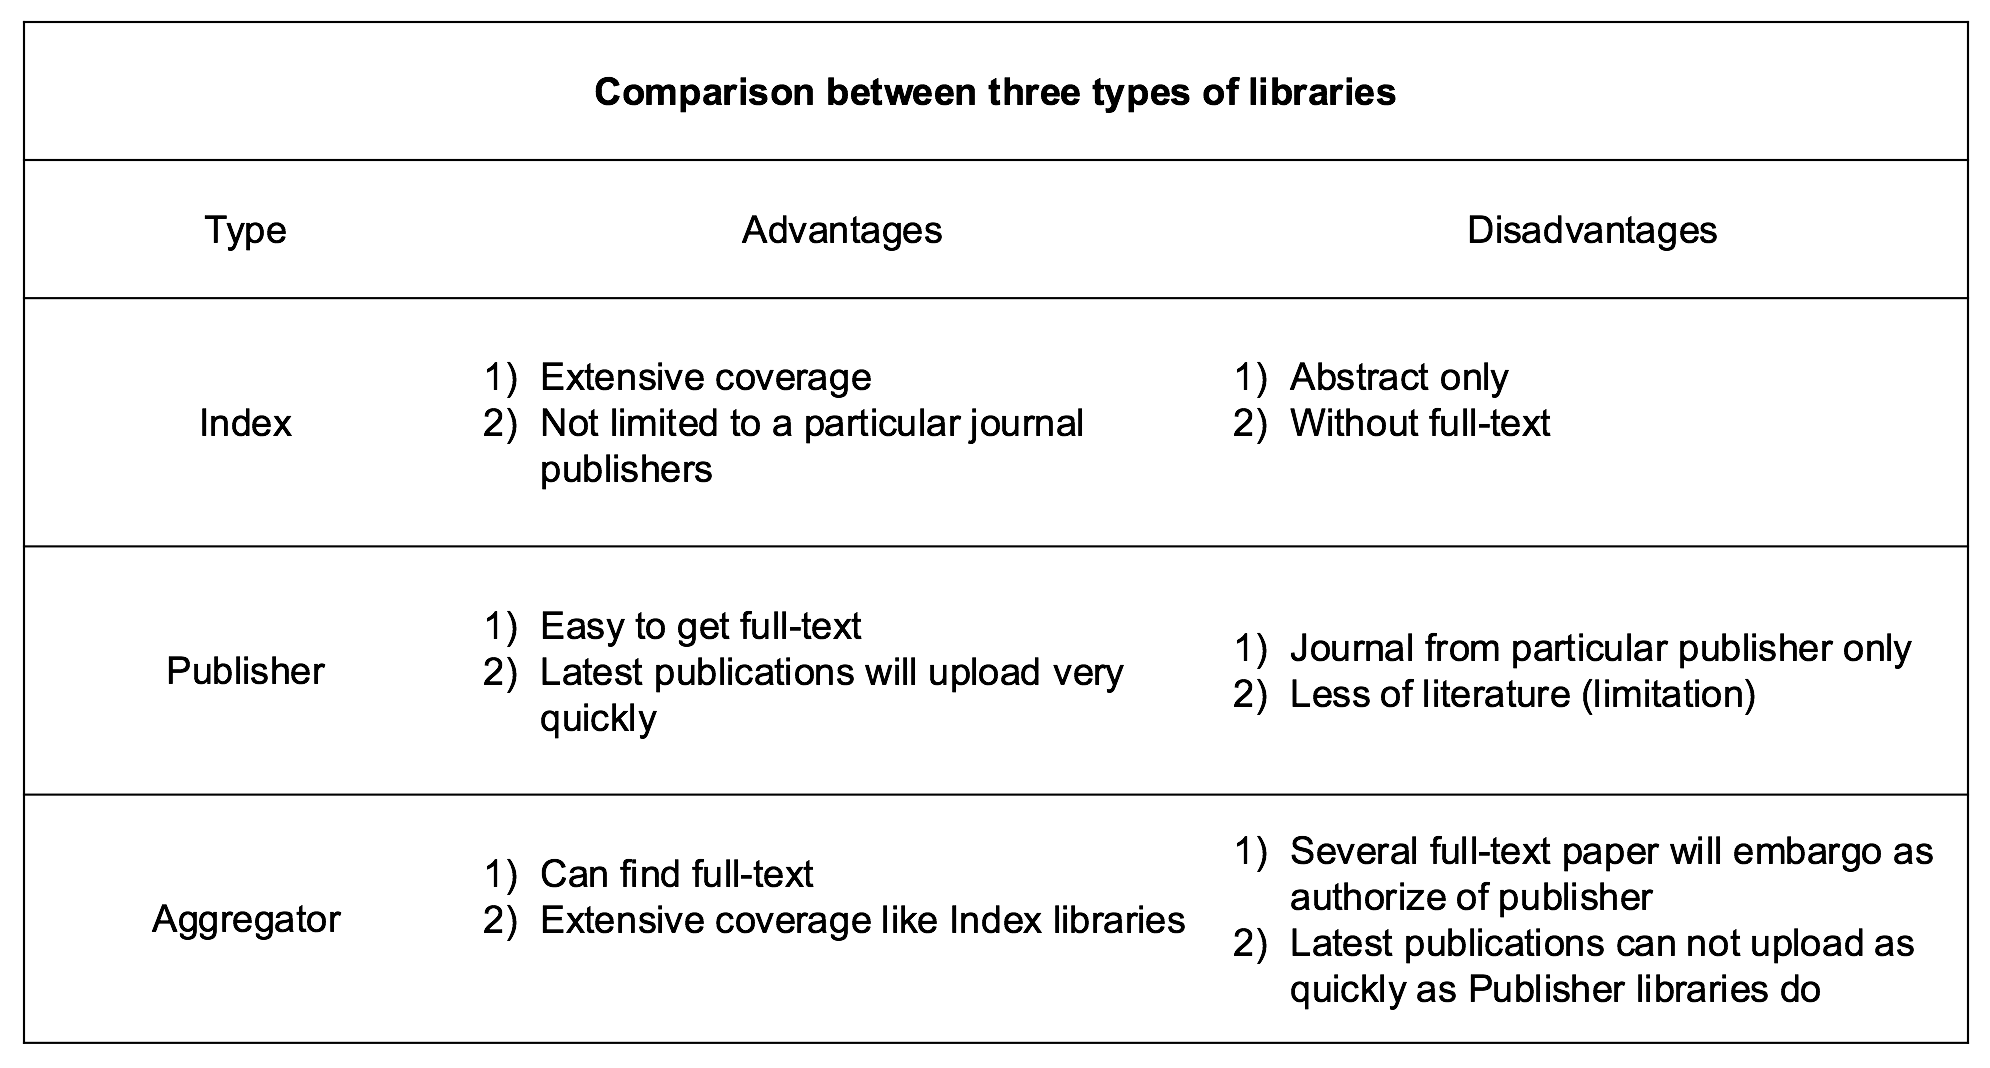
\includegraphics[width=0.8\textwidth]{Wolverine_Background_Chart_1}
	\end{center}
	\caption{Comparison between three types of libraries.\label{WBC1}}
\end{figure*}
\newpage
